\section{Code generation}
\subsection{Double Roof}
\begin{figure}[h]
	\begin{center}
		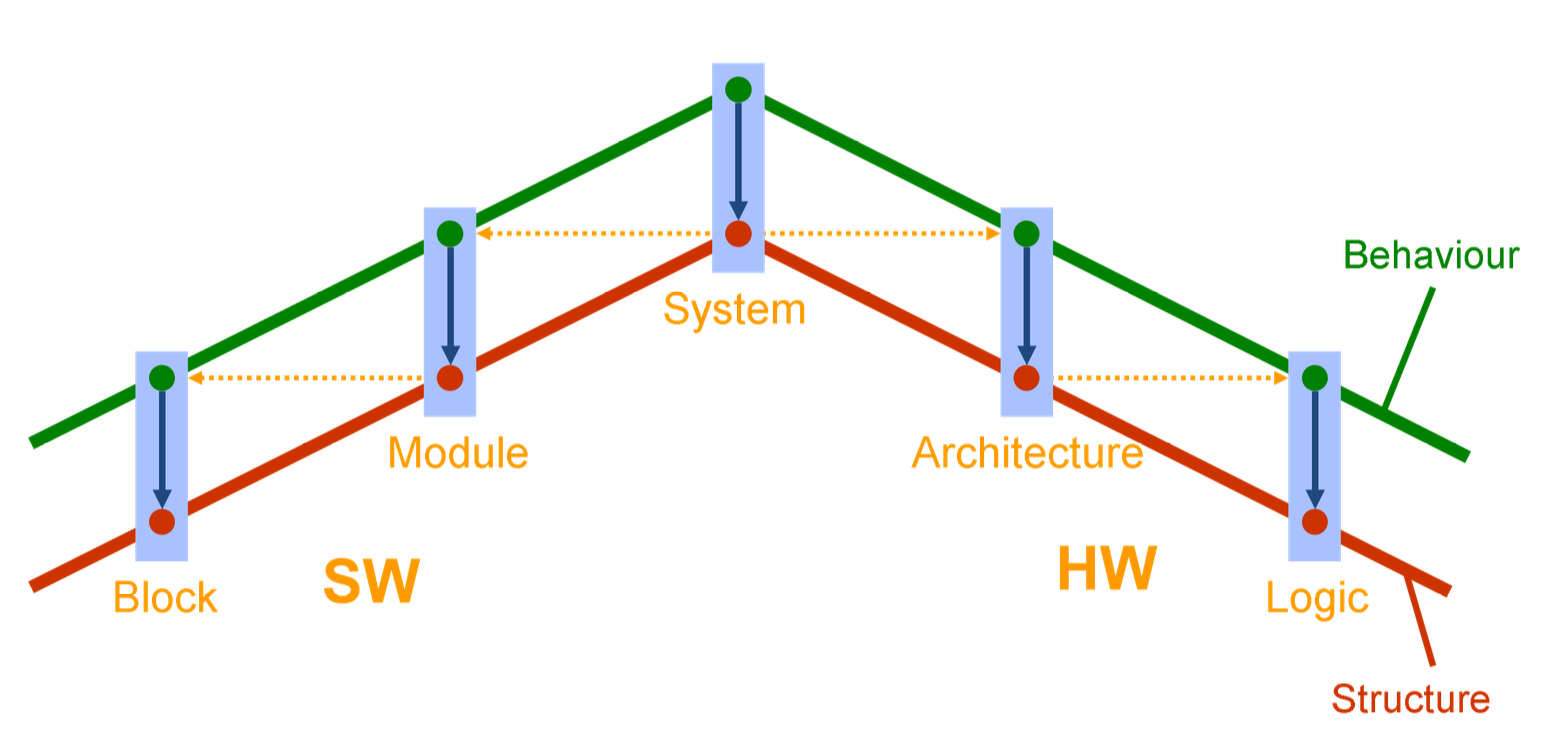
\includegraphics[width=0.5\textwidth]{images/Double_roof.png}
		\caption{Double Roof}
		\label{fig:double_roof}
	\end{center}
\end{figure}
\subsection{Compiler - Basics}
\begin{figure}[h]
	\begin{center}
	\begin{subfigure}[b]{0.4\textwidth}
		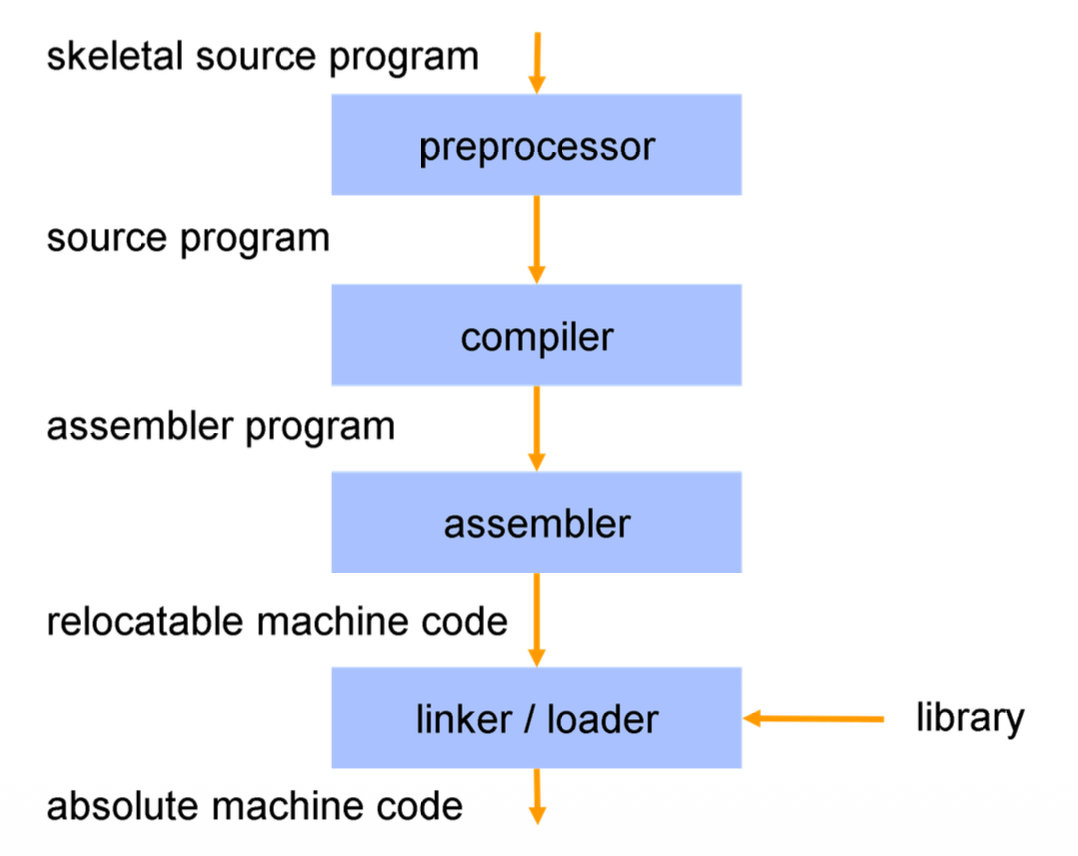
\includegraphics[width=\textwidth]{images/Compilation_process.png}
		\caption{Compilation Process}
		\label{fig:comp_process}
	\end{subfigure}
	\hfill
	\begin{subfigure}[b]{0.5\textwidth}
		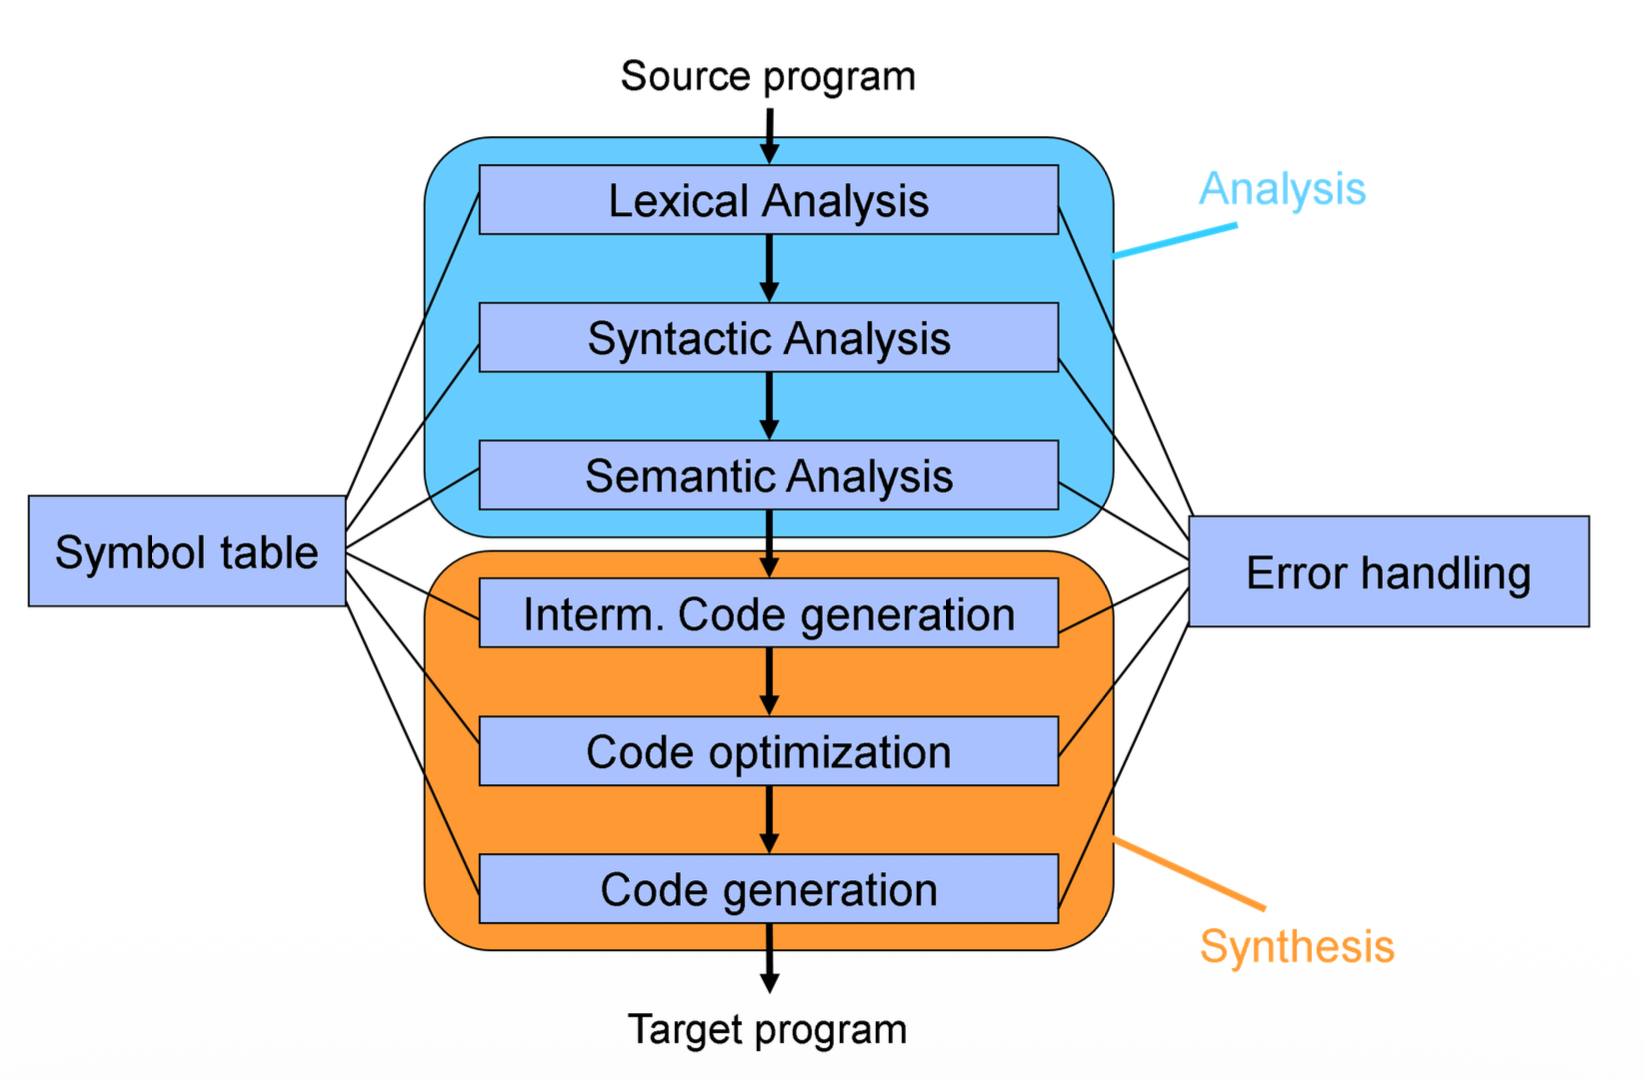
\includegraphics[width=\textwidth]{images/Compilor_phases.png}
		\caption{Compilation Process}
		\label{fig:comp_process}
	\end{subfigure}
	\caption{Compiler}
\end{center}
\end{figure}

\subsubsection{Analysis}
\begin{itemize}
	\item Lexical Analysis
\begin{itemize}
	\item scan source program and decompose it into symbols 
	\item regular expression: recognition through finite automata 
\end{itemize}
\item syntactic analysis
\begin{itemize}
	\item parse sequences of symbols and determine clauses
	\item clauses are described by a context free grammar
\begin{itemize}
	\item Z $\rightarrow$ Identifier $:=$ A
	\item A $\rightarrow$ A + A $|$ A * A $|$ Identifier $|$ Number
\end{itemize}
\end{itemize}
\item semantic analysis
\begin{itemize}
	\item assure that the pieces fit together semantically
	\item Example: type conversion
\end{itemize}
\end{itemize}

\begin{figure}[h]
	\begin{center}
		\begin{subfigure}[b]{0.5\textwidth}
			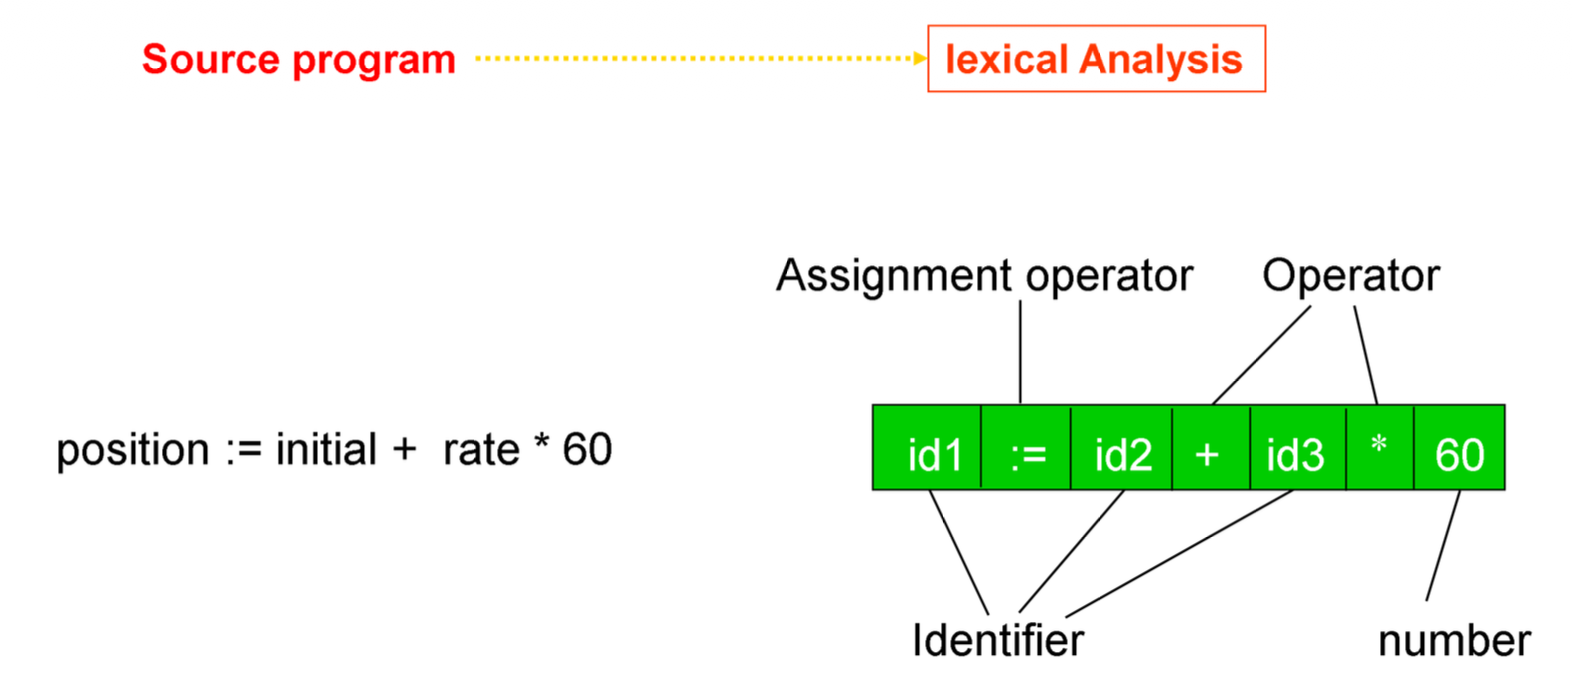
\includegraphics[width=\textwidth]{images/Analysis_1.png}
		\end{subfigure}
		\hfill
		\begin{subfigure}[b]{0.4\textwidth}
			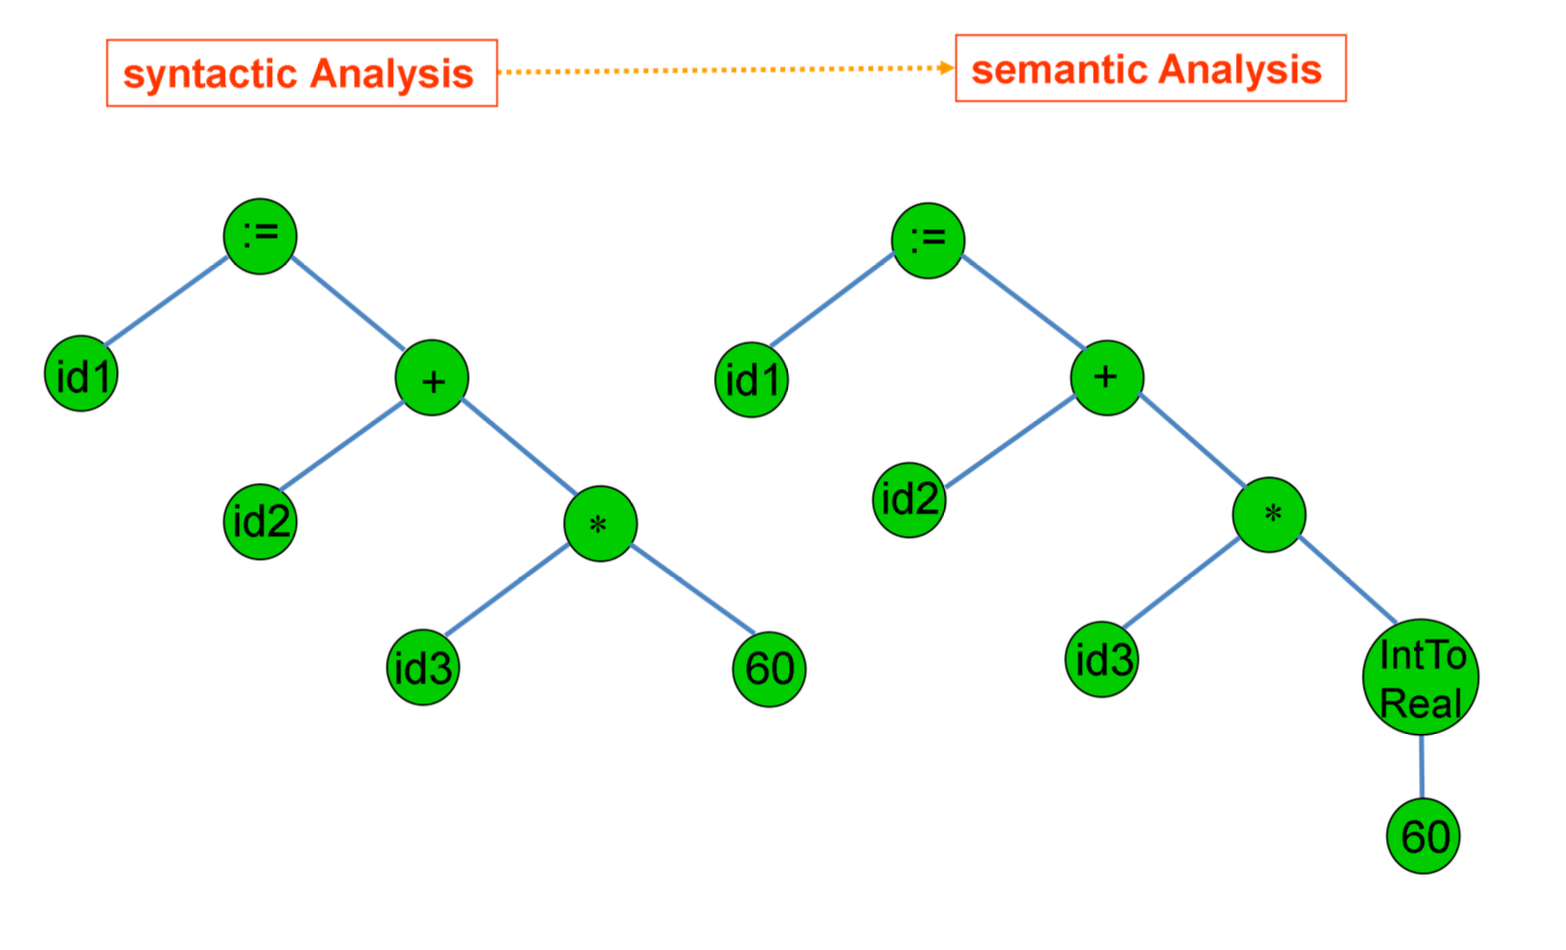
\includegraphics[width=\textwidth]{images/Analysis_2.png}			
		\end{subfigure}
		\caption{Analysis Example}
		\label{fig:analysis}
	\end{center}
\end{figure}

\subsubsection{Synthesis}
\begin{itemize}
	\item Generation of intermediate code
\begin{itemize}
	\item machine independent $\rightarrow$ retargeting easier
	\item easy to generate
	\item easy to be translated 
\end{itemize}
\item Optimization
\begin{itemize}
	\item General-purpose processors: fast code, fast translation
	\item Special processors: fast code, compact code, small memory image
	\item of intermediate code or of target code
\end{itemize}
\item Code generation
\end{itemize}

\begin{figure}[h]
	\begin{center}
		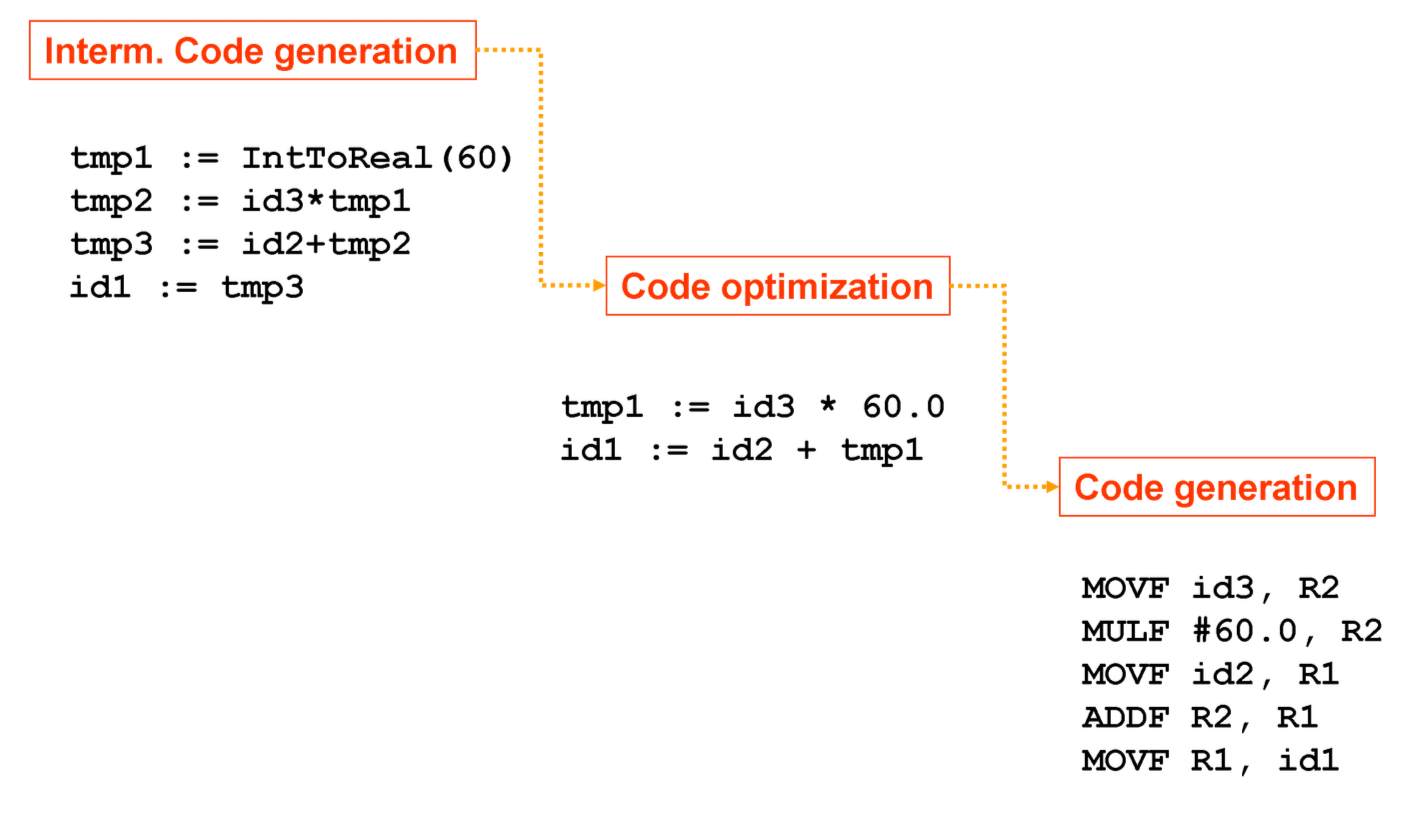
\includegraphics[width=0.5\textwidth]{images/Synthesis.png}
		\caption{Synthesis Example}
		\label{fig:synthesis}
	\end{center}
\end{figure}

\subsubsection{Syntax Tree abd DAG}
\begin{figure}[h]
	\begin{center}
		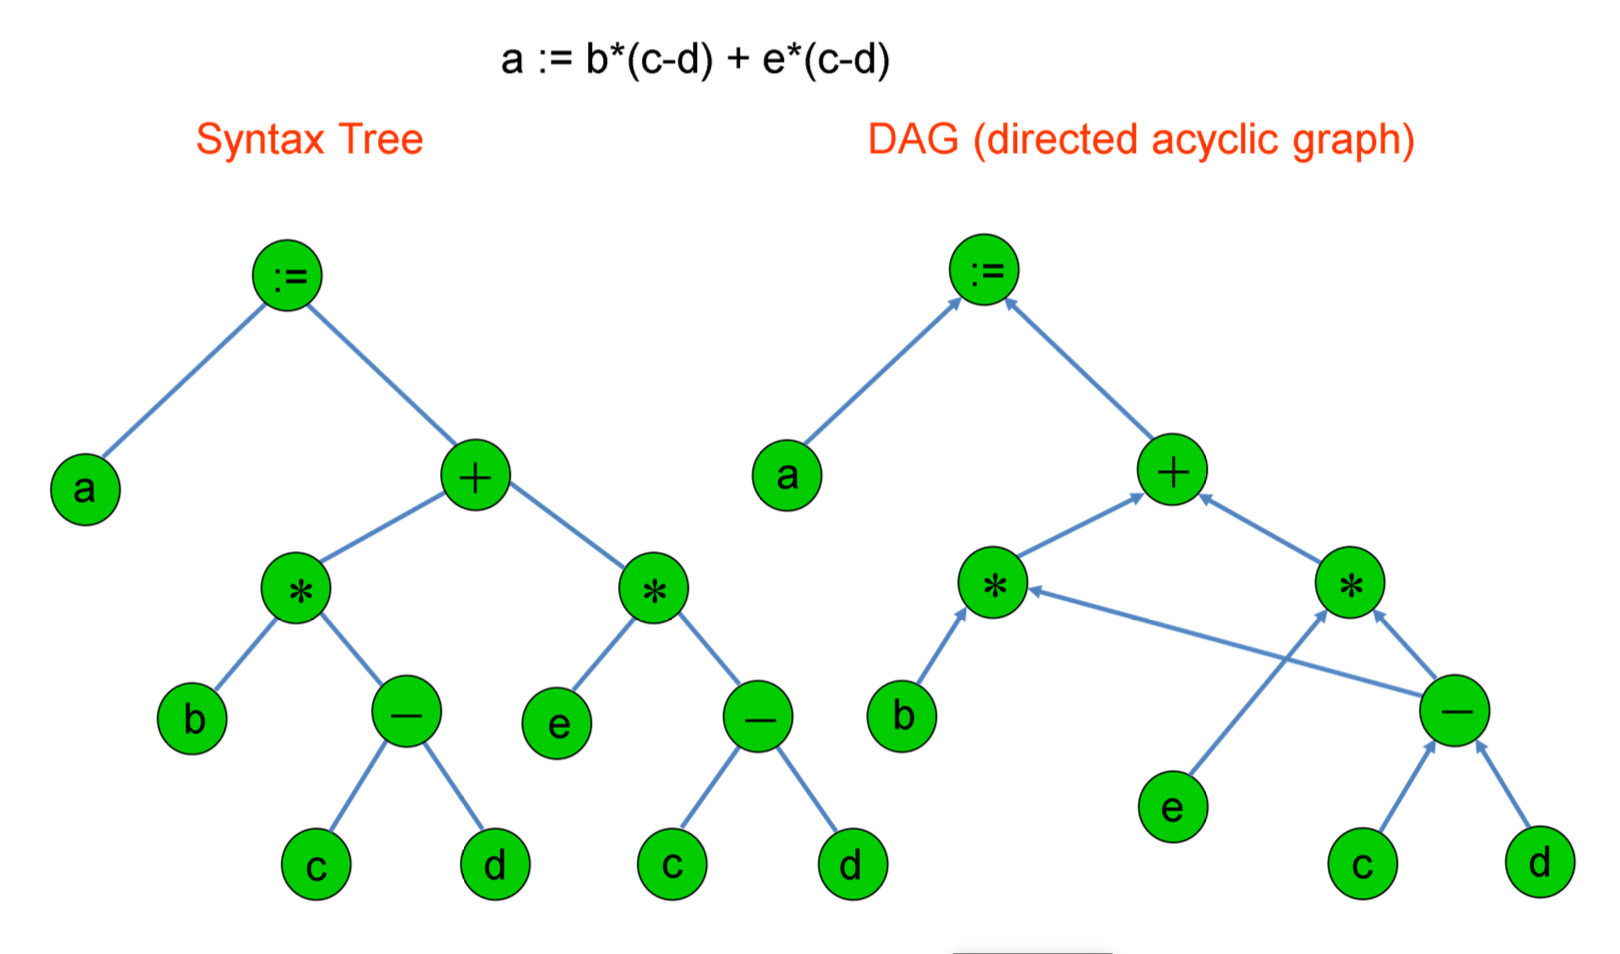
\includegraphics[width=0.5\textwidth]{images/Syn_and_DAG.png}
		\caption{Syntax Tree and DAG}
		\label{fig:syn_and_DAG}
	\end{center}
\end{figure}


\subsubsection{3-Address Code}
\begin{itemize}
	\item Instructions
\begin{itemize}
	\item maximum 3 addresses (2 operands, 1 result)
	\item maximum 2 operants
\end{itemize}
\item Assignments
\begin{itemize}
	\item \begin{verbatim} x := y op z\end{verbatim}
	\item \begin{verbatim} x := op y\end{verbatim}
	\item \begin{verbatim} x := y\end{verbatim}
	\item \begin{verbatim} x := y[i]\end{verbatim}
	\item \begin{verbatim} x[i] := y\end{verbatim}
	\item \begin{verbatim} x := &y\end{verbatim}
	\item \begin{verbatim} y := *x\end{verbatim}
	\item \begin{verbatim} *x := y\end{verbatim}
\end{itemize}
\item Control flow
\begin{itemize}
	\item \begin{verbatim} goto L\end{verbatim} 
	\item \begin{verbatim} if x relop y goto L	\end{verbatim}
\end{itemize}
\item Sub programs
\begin{itemize}
	\item \begin{verbatim} param x\end{verbatim}
	\item \begin{verbatim} call p,n\end{verbatim}
	\item \begin{verbatim} return y\end{verbatim}
\end{itemize}
\item Advantages
\begin{itemize}
	\item resolution of lengthy expressions and nested loops
	\item temporary names allow for easy reordering
	\item represents already a valid schedule
\end{itemize}
\item Definition
\begin{itemize}
	\item \begin{verbatim} x := y op z\end{verbatim}
	\item defines x and uses y and z
\end{itemize}
\end{itemize}

\begin{figure}[h]
	\begin{center}
		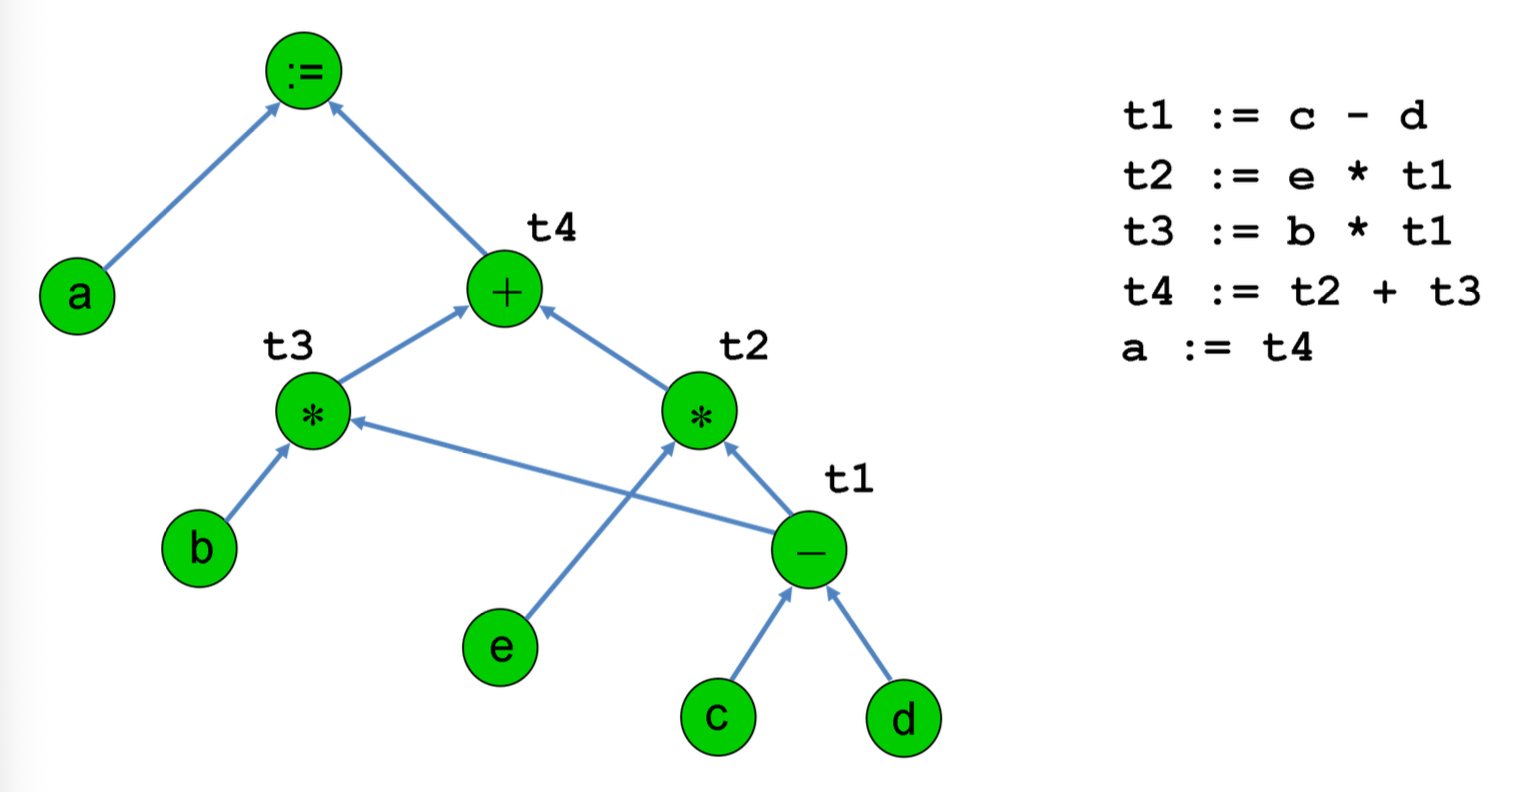
\includegraphics[width=0.5\textwidth]{images/3-address.png}
		\caption{Generation of 3-address-code from DAG}
		\label{fig:3-address}
	\end{center}
\end{figure}

\subsubsection{Basic Block}
Definition: A basic block is a sequence of consecutive instructions in which the control flow enters at the beginning and leaves at the end without branching except at the end.

Sequence of 3-address instructions $\rightarrow$ set of basic block:
\begin{enumerate}
  \item Determine block start points:
\begin{itemize}
	\item the first instruction
	\item targets of branch and jump instructions
	\item instructions directly following a branch or jump instruction
\end{itemize}
\item Determination of basic blocks
\begin{itemize}
	\item each basic block includes its block start point
	\item includes all instructions (but excluding) the next block start point or until the program ends
\end{itemize}

\end{enumerate}

\subsubsection{CFG and DAG for basic blocks}
\begin{figure}[h]
	\begin{center}
	\begin{subfigure}[b]{0.45\textwidth}
		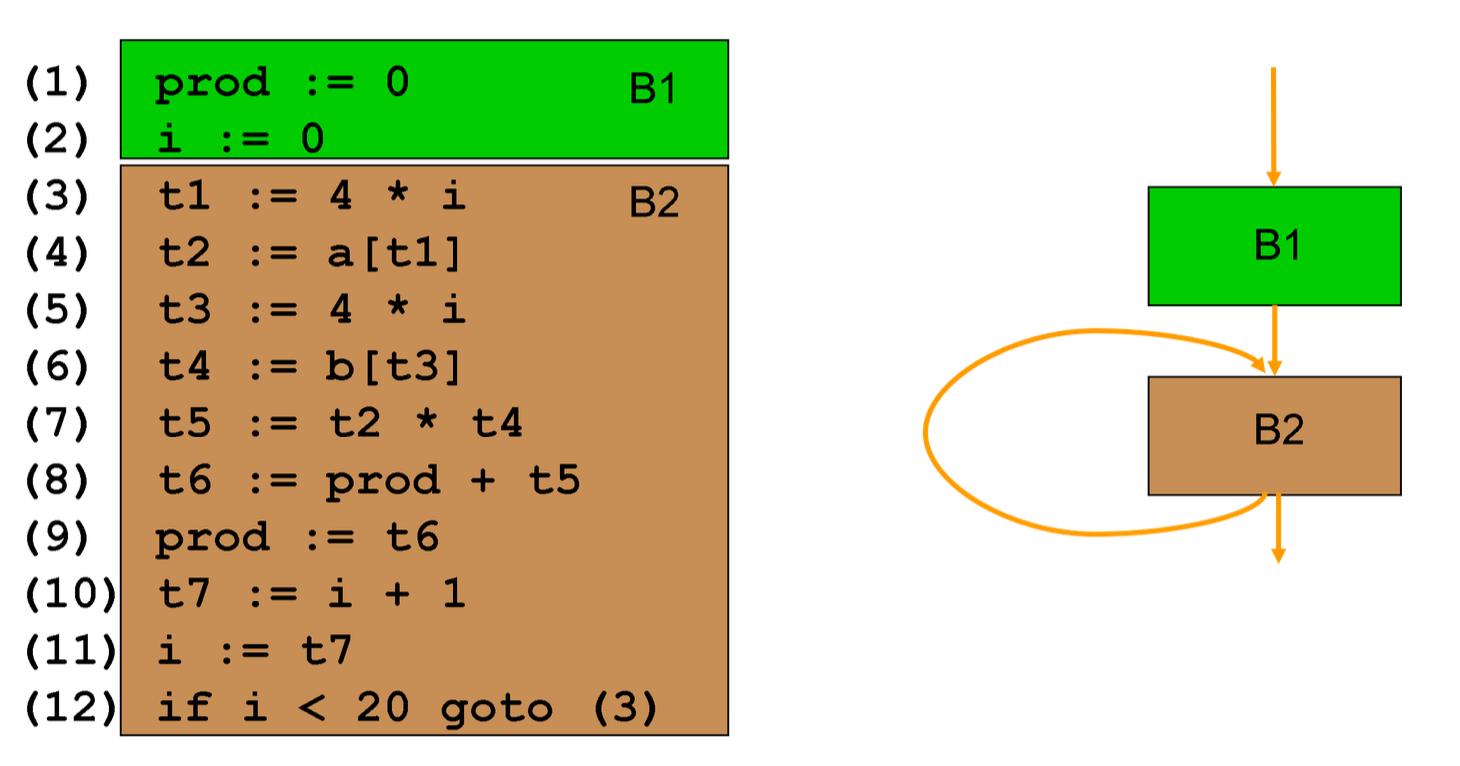
\includegraphics[width=\textwidth]{images/Degen_CFG.png}
		\caption{Degenerated Control Flow Graph}
		\label{fig:degen_CFG}
	\end{subfigure}
	\hfill
	\begin{subfigure}[b]{0.45\textwidth}
		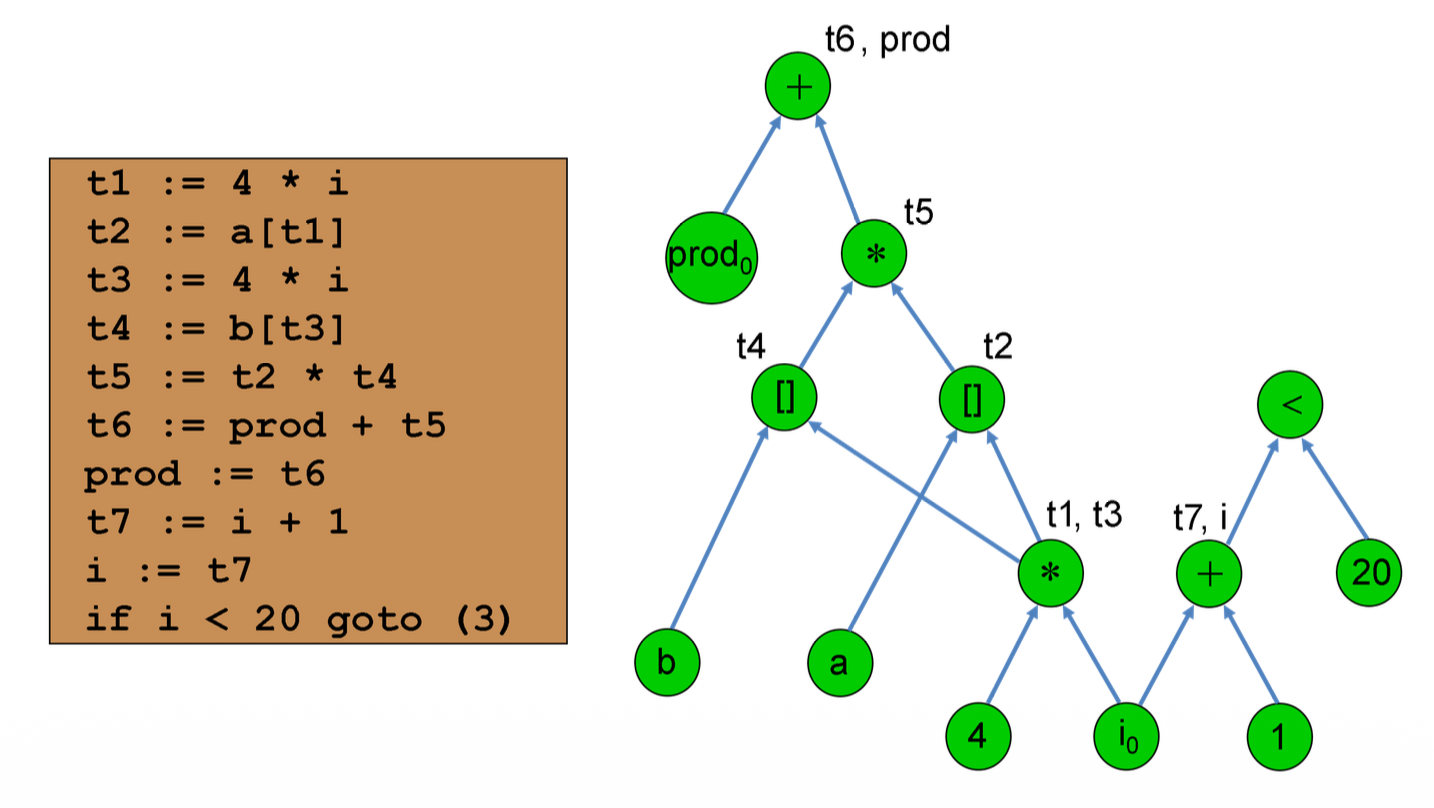
\includegraphics[width=\textwidth]{images/DAG_bb.png}
		\caption{Directed acyclic graph}
		\label{fig:DAG_basic_block}
	\end{subfigure}
	\caption{CFG and DAG for basic blocks}
	\end{center}
\end{figure}

\subsection{Code generation}
\begin{itemize}
	\item Requirements
\begin{itemize}
	\item correct code
	\item efficient code
	\item efficient code generation
\end{itemize}
\item Code generation = Software synthesis
\begin{itemize}
	\item Allocation: often given
	\item Binding:
\begin{itemize}
	\item Register allocation, register binding
	\item Code (instruction) selection
\end{itemize}
\item Scheduling
\begin{itemize}
	\item Instruction sequencing
\end{itemize} 
\end{itemize}
\item Goal: efficient register usage
\begin{itemize}
	\item instructions on register operands typically shorter and faster as instructions with memory operands
\end{itemize}
\item Register allocation, register binding
\begin{itemize}
	\item determine at each point of the program the set of variables hat shall be stored in a register
	\item bind each variable to a physical register
	\item optimal register binding in a NP-complete problem
	\item additional constrains given by special registers of the CPU architecture, compiler and operating system
\end{itemize}
\end{itemize}

\subsubsection{Code (Instruction) Selection}
\begin{itemize}
	\item Code pattern for implementing a 3-address instruction [\cref{fig:3-addres_to_assembler}]
	\item Problems
\begin{itemize}
	\item often inefficient code $\rightarrow$ Code optimization
	\item There may be many alternative instructions
	\item some instructions are only executable on certain registers
	\item exploitation of special processor properties   
\end{itemize}
\end{itemize}

\begin{figure}[h]
	\begin{center}
		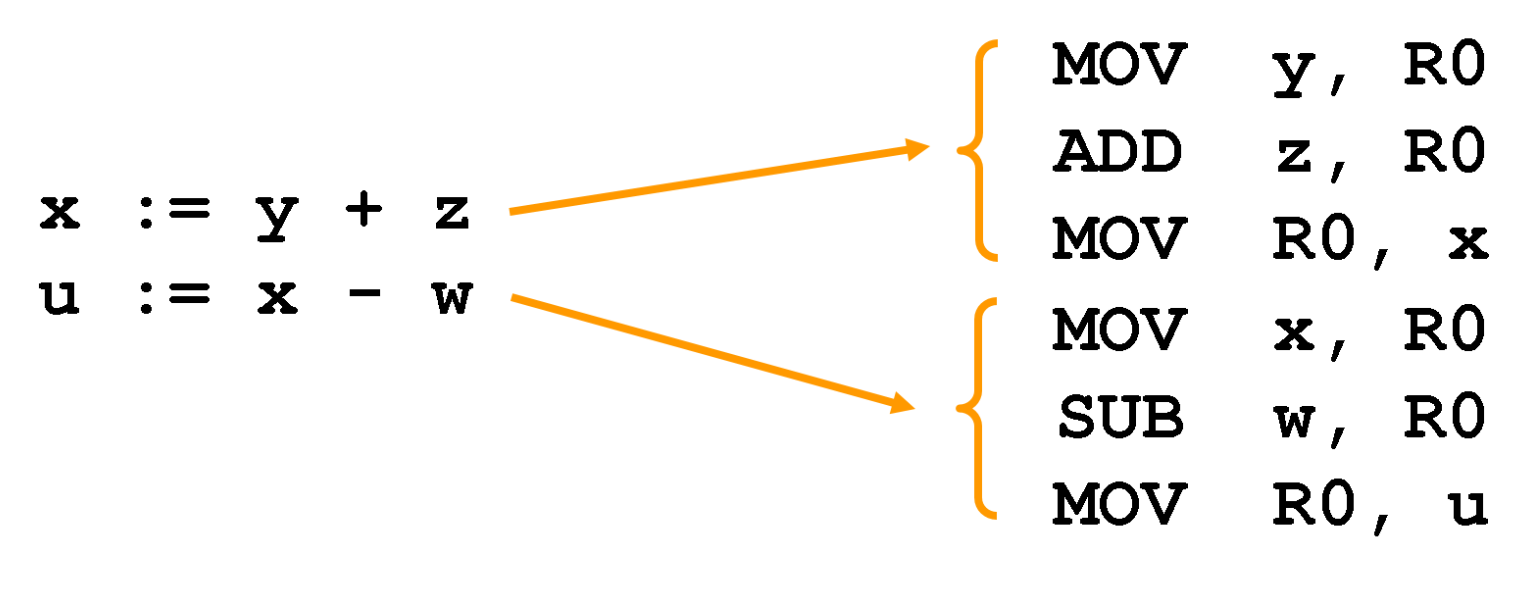
\includegraphics[width=0.5\textwidth]{images/Code_selection.png}
		\caption{3-address to assembler}
		\label{fig:3-addres_to_assembler}
	\end{center}
\end{figure}

\subsubsection{Scheduling}
Goal: efficient instruction execution sequences, as short as possible, using few registers

\begin{figure}[h]
	\begin{center}
		\begin{subfigure}[b]{0.55\textwidth}
			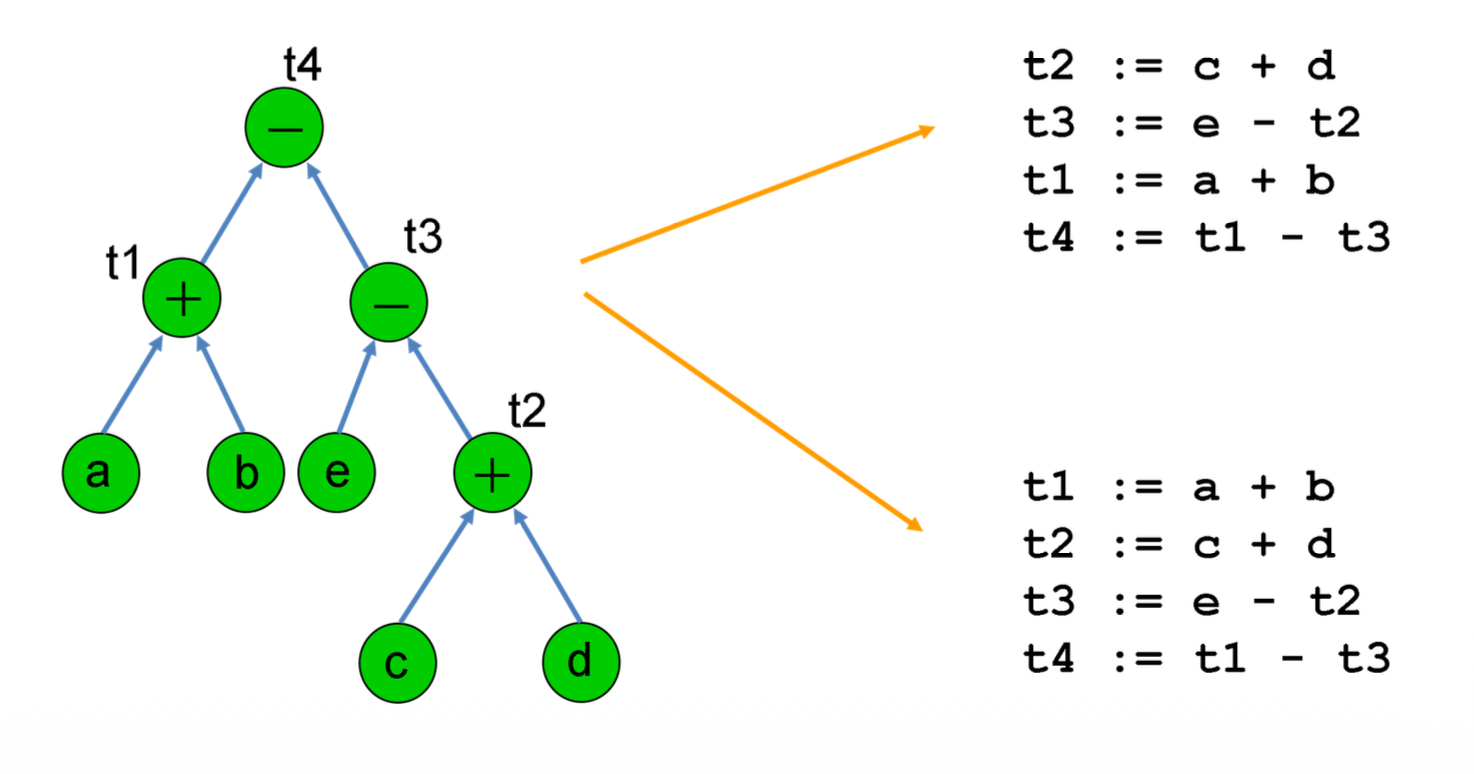
\includegraphics[width=\textwidth]{images/Scheduling_1.png}
		\end{subfigure}
		\hfill
		\begin{subfigure}[b]{0.35\textwidth}
			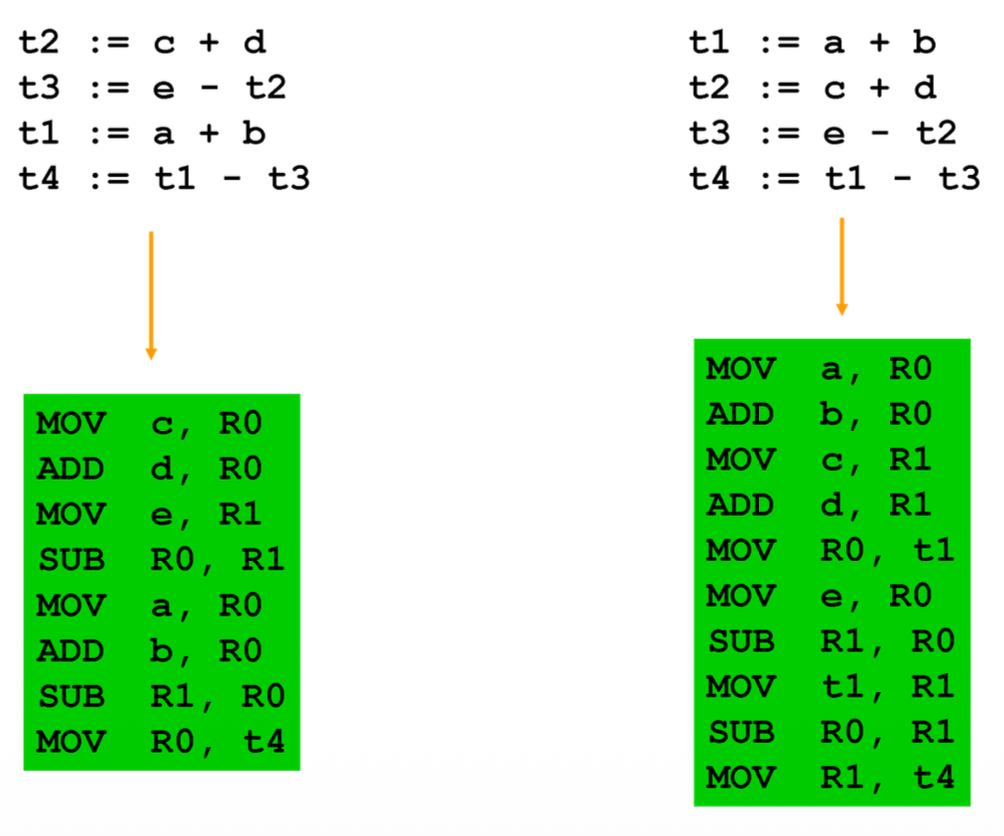
\includegraphics[width=\textwidth]{images/Scheduling_2.png}
		\end{subfigure}
		\caption{Scheduling differences}
		\label{fig:scheduling}
	\end{center}
\end{figure}

\subsubsection{Register allocation}
\begin{itemize}
	\item global register allocation
\begin{itemize}
	\item reserve a certain number of registers
\begin{itemize}
	\item for global variables
	\item for loop variables
	\item for variables in basic blocks
\end{itemize}
	\item user-defined register allocation
\begin{itemize}
	\item E.g. in programming language C: 
	\begin{verbatim}register int i;\end{verbatim}
\end{itemize}
\end{itemize}
	\item Usage counters
	\item Register assignment through graph coloring
\end{itemize}

\subsubsection{Usage Counters}
\begin{itemize}
	\item Let a loop \verb|L| be composed of multiple basic blocks
	\item In case a variable \verb|a| is kept in a register during execution of Loop \verb|L|, we obtain cost savings
\begin{itemize}
	\item 1 cost unit for each reference to \verb|a|
\begin{itemize}
	\item \verb|ADD R0, R1| (cost 1) instead of \verb|ADD a, R1| (cost 2)
\end{itemize}
	\item 2 cost units for each basic block, if \verb|a| is defined in the basic block and active still thereafter
\begin{itemize}
	\item no store necessary (\verb|MOV R0, a|)
\end{itemize}
\end{itemize}
	\item Cost savings for the whole loop
$$
	\sum_{B\in L} (\text{verwendet}(a, B)+2\cdot \text{aktiv}(a, B))
$$
\begin{itemize}
	\item verwendet($a, B$) denotes the number of uses of $a$ in basic block $B$ before potentially being defined therein 
	\item aktiv($a, B$) equals $1$, if $a$ has been defined in $B$ and is active at the end of $B$; else $0$
\end{itemize}
	\item Approximation of cost savings for assumption that
\begin{itemize}
	\item all basic blocks are executed equally often
	\item loop will be executed often
\end{itemize}
\end{itemize}

\begin{figure}
	\begin{center}
		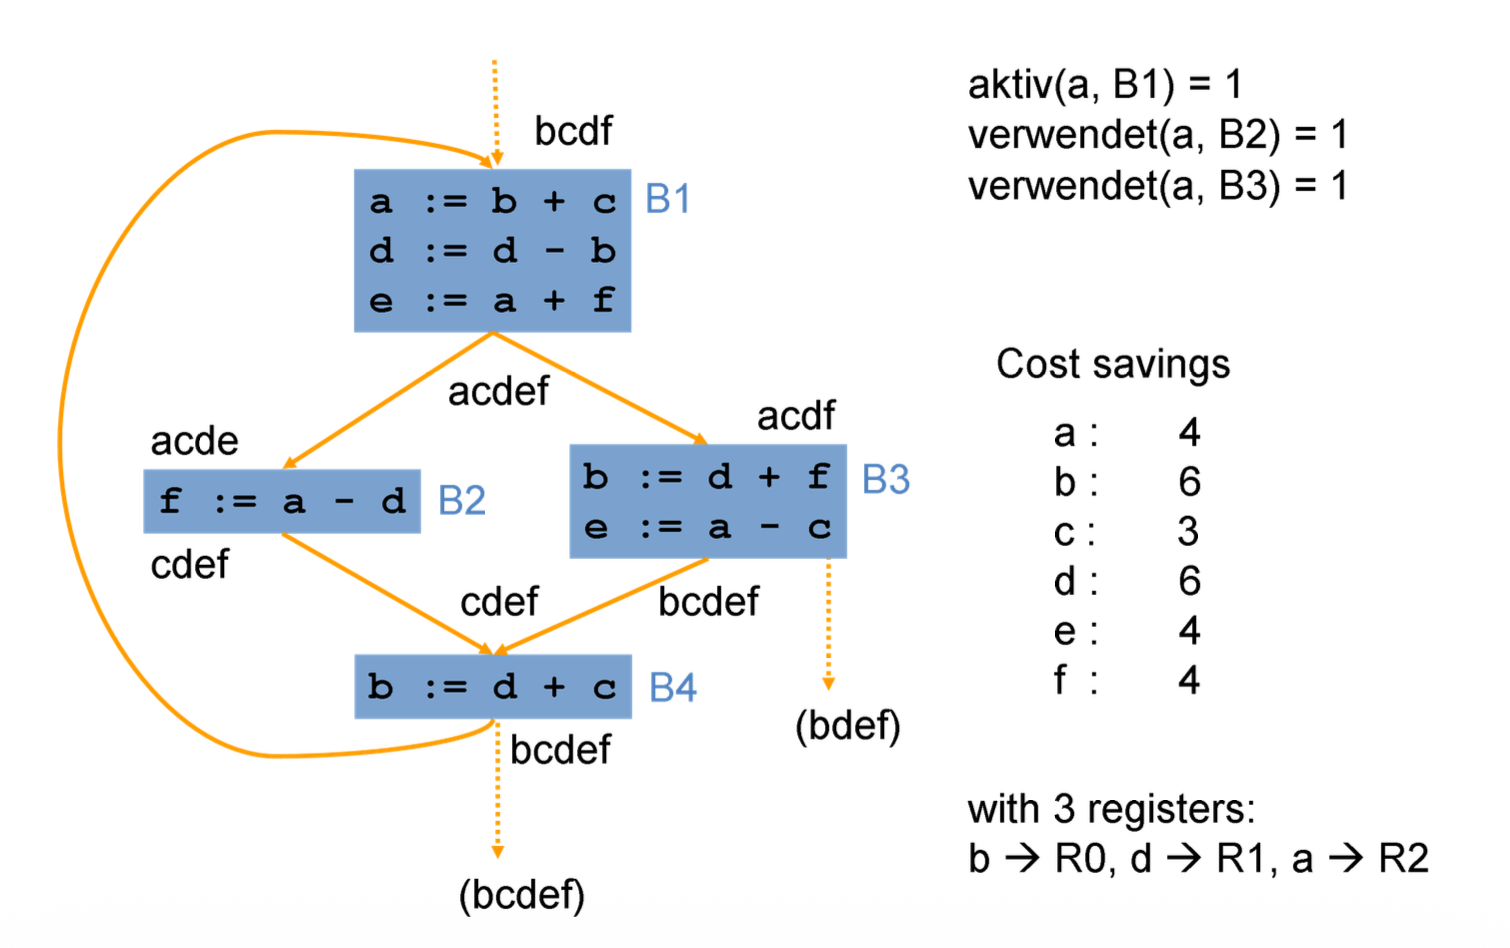
\includegraphics[width=0.5\textwidth]{images/Usage_counter.png}
		\caption{
			Usage Counter - Example \\
			Variables in brackets are given. Start from bottom. Variables below basic block remain active. Basic block depends on variables above.  
		}
	\end{center}
\end{figure}

\subsubsection{Register Binding using Graph Coloring}
\begin{itemize}
	\item Flow
\begin{enumerate}
  \item Apply code generation assuming unbounded number of available registers, i.e. each variable is assigned to a unique symbolic register
  \item Determine the life time of each variable 
  \item Construct a conflict graph
  \item Mapping of symbolic registers onto physical registers through graph coloring 
\end{enumerate}
\item Nodes represent the symbolic registers and edges represent conflict between variables 
\item Heuristics: Is a graph $G$ colorable with $I$ colors?
\begin{enumerate}
  \item Determine a node $v_i \in G$ of degree Grad($v_i$)$<I$
  \item Eliminate $v_i$ and all incident edges to obtain a graph $G'$
  \item If $G'=\emptyset$:
\begin{itemize}
	\item $I$-coloring possible
\end{itemize}
  If all nodes in $G'$ have degree $\geq I$:
  \begin{itemize}
	\item $I$-coloring not possible
\end{itemize}
  $G=G'$ and goto 1
\end{enumerate}

\end{itemize}

\begin{figure}[ht]
	\begin{center}
		\begin{subfigure}[b]{0.35\textwidth}
			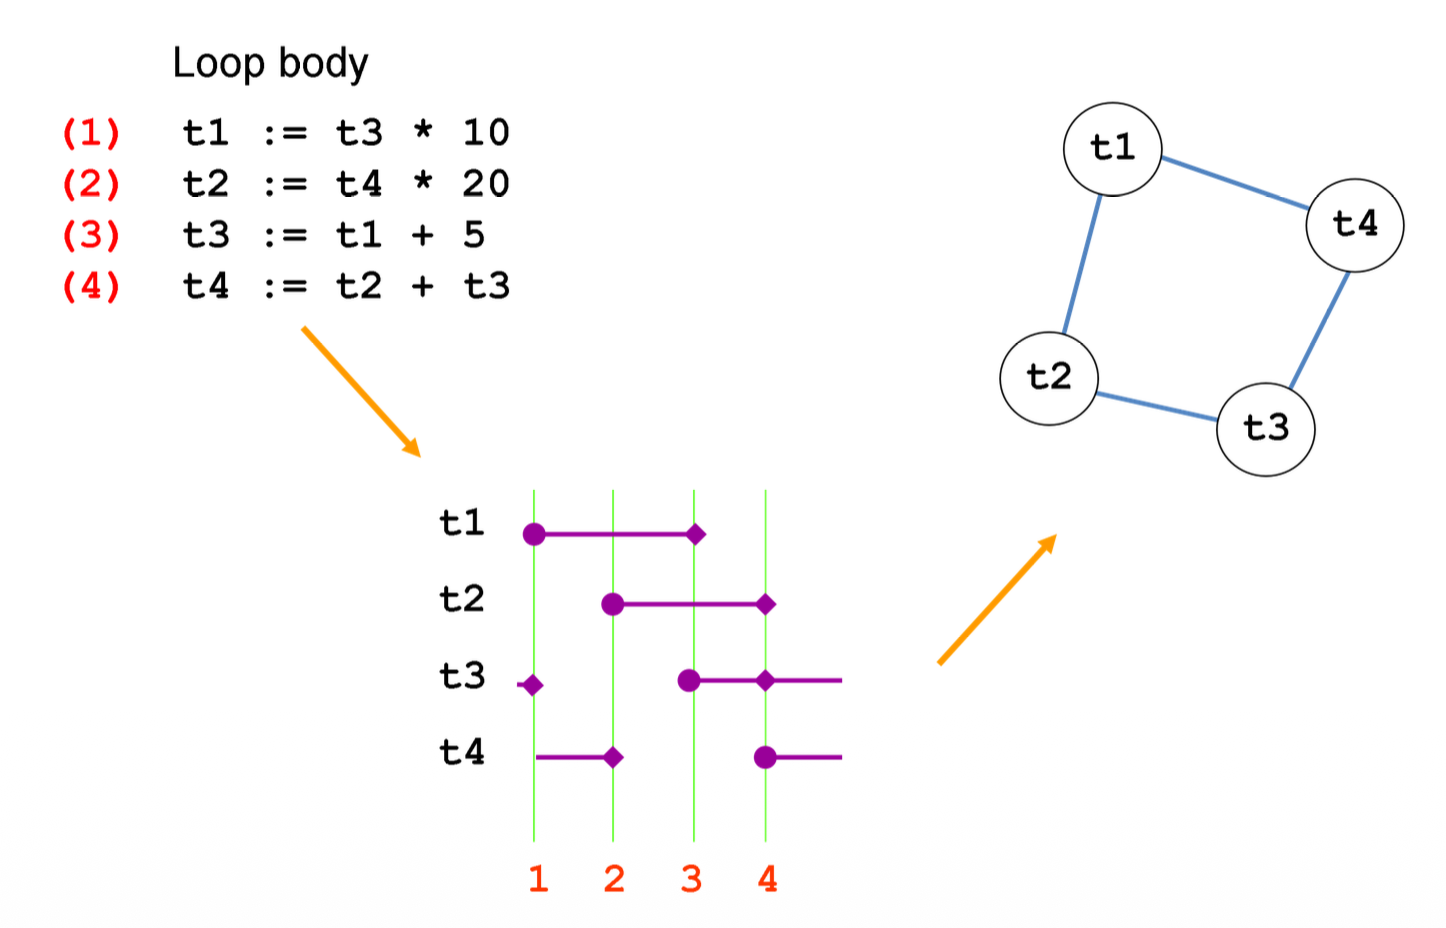
\includegraphics[width=\textwidth]{images/Register_conflict_graph_1.png}
		\end{subfigure}
		\hfill
		\begin{subfigure}[b]{0.55\textwidth}
			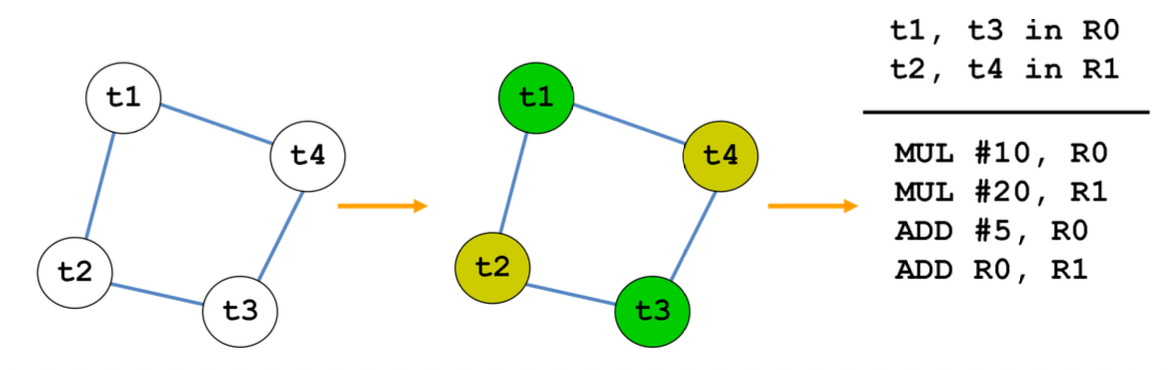
\includegraphics[width=\textwidth]{images/Register_conflict_graph_2.png}			
		\end{subfigure}
		\caption{Register conflict graph - Example}
		\label{fig:register_conflict_graph}
	\end{center}
\end{figure}

\begin{figure}[ht]
	\begin{center}
		\begin{subfigure}[b]{0.5\textwidth}
			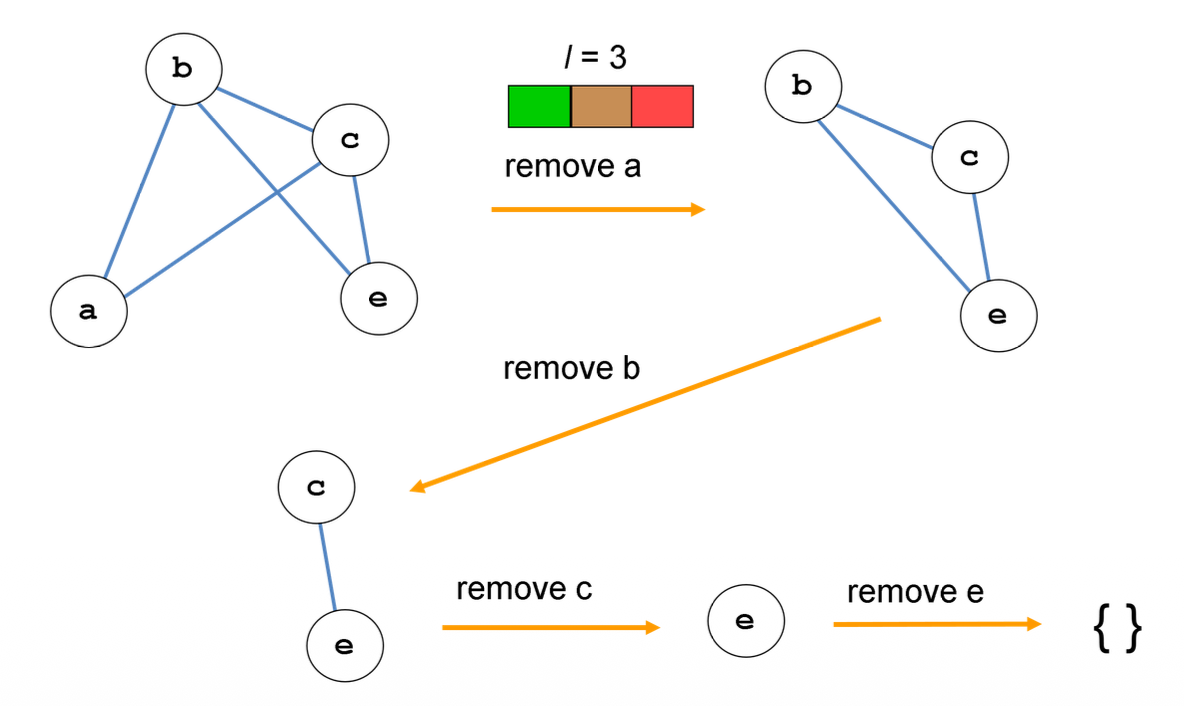
\includegraphics[width=\textwidth]{images/Register_conflict_graph_3.png}
		\end{subfigure}
		\hfill
		\begin{subfigure}[b]{0.4\textwidth}
			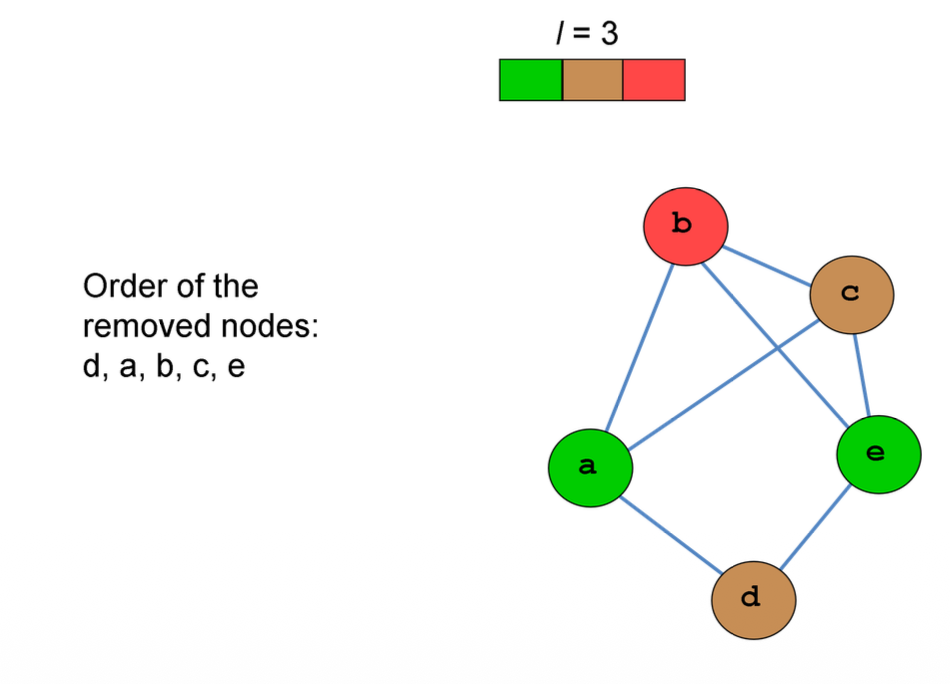
\includegraphics[width=\textwidth]{images/Register_conflict_graph_4.png}	
		\end{subfigure}
		\caption{Graph coloring - Example}
		\label{fig:graph_coloring}
	\end{center}
\end{figure}

\subsection{Code Generation for DAGs}
\begin{itemize}
	\item The order of evaluation of the nodes pf a DAG may have a great influence on the number of required instructions
	\item Heuristic for determination of a feasible evaluation order:
\end{itemize}
\begin{verbatim}
	while there exists any non-ranked inner node do
	    choose a node n whose parents have been ranked and rank it
	    while the furthest left child m of n has no unranked parents and is no leaf do
	        rank node m
	        n <- m
	    end while
	 end while   
\end{verbatim}  

\begin{itemize}
	\item For a DAG with $n$ nodes that is a tree there is an algorithm that determines optimal code in time $\BigO(n)$
	\item common subexpressions
\begin{itemize}
	\item If the DAG is not a tree $\rightarrow$ split the DAG at nodes that represent common subexpressions and generate optimal code for each part
\end{itemize}
\end{itemize}

\subsubsection{Dynamic Programming}
\begin{itemize}
	\item Machine model extended to more complex instructions
\begin{itemize}
	\item $n$ Register \verb|R0...Rn-1|
	\item Instructions \verb|Ri:=E| \\
			E is an arbitrary expression including registers and memory locations as operants
	\item  In case E contains multiple registers, then Ri must be one of them
	\item Load: \verb|Ri:=M|, Store: \verb|M:=Ri|, Move/Copy: \verb|Ri:=Rj|
\end{itemize}
	\item Examples
\begin{itemize}
	\item \verb|ADD R0, R1| $\rightarrow$ \verb|R1:=R1+R0|
	\item \verb|ADD *R0, R1| $\rightarrow$ \verb|R1:=R1 + ind R0|
	\item \verb|SUB a, R0| $\rightarrow$ \verb|R0:=R0-a|
\end{itemize}
	\item Optimal code for \verb|E=(T1 op T2)|:
\begin{enumerate}
	\item Optimal code for \verb|T1|, \verb|T2|
	\item Either \verb|T1, T2, op| or \verb|T2, T1, op|
\end{enumerate}
	\item Method runs in 3 phases
\begin{enumerate}
    \item Computation of cost vectors
    \item Determination of execution orders
    \item Generation of target code
\end{enumerate}
	\item Determination of cost vectors for each node $n$ (bottom up)
\begin{itemize}
	\item $C[i]$ optimal cost for computing $n$ with $i$ available registers
	\item $C[0]$ optimal cost for computing $n$ when result is stored in memory
\end{itemize}
\end{itemize}

\subsection{Code Optimization}
\begin{itemize}
	\item Transformations possible on either intermediate code or on target code
	\item Peephole Optimization
\begin{itemize}
	\item small window is moved over code
	\item multiple runs, as one optimization may trigger anotherone
\end{itemize}
	\item Local Optimization
\begin{itemize}
	\item Transformation on basic blocks 
\end{itemize}
	\item Global Optimization
\begin{itemize}
	\item Transformations affecting multiple basic blocks
\end{itemize}
\end{itemize}

\subsubsection{Peephole Optimization}
\begin{itemize}
	\item Elimination of redundant assignments
\begin{verbatim}
(1) MOV R0, a
(2) MOV a, R0
\end{verbatim}
\begin{center}$\downarrow$\end{center}
\begin{verbatim}
(1) MOV R0, a
\end{verbatim}
	\item Algebraic simplification \\
\verb|x := y + 0 * a;| $\rightarrow$ \verb|x := y;|
	\item Control flow optimization
\begin{verbatim}
	(1)     goto L1
	(2) L2  goto L2
\end{verbatim}
\begin{center}$\downarrow$\end{center}
\begin{verbatim}
	(1)     goto L2
	(2) L1  goto L2 
\end{verbatim}
	\item Operator (strength) reduction \\
\verb|x := y*8;| $\rightarrow$ \verb|x := y << 3;| \\
\verb|x := y**2;| $\rightarrow$ \verb|x := y*y;|
	\item Common subexpression elimination
\begin{verbatim}
	(1) a := b + c
	(2) b := a - d
	(3) c := b + c
	(4) d := a - d
\end{verbatim} 
\begin{center}$\downarrow$\end{center}
\begin{verbatim}
	(1) a := b + c
	(2) b := a - d
	(3) c := a
	(4) d := b
\end{verbatim}
	\item Variable renaming \\
\verb|t := b + c| $\rightarrow$ \verb|u := b + c|
	\item Instruction interchange
\begin{verbatim}
	t1 := b + c
	t2 := x + y
\end{verbatim}
\begin{center}$\downarrow$\end{center}
\begin{verbatim}
	t2 := x + y
	t1 := b + c
\end{verbatim}
\end{itemize}

\subsubsection{Global Optimization}
\begin{itemize}
	\item Passive code elimination
\begin{itemize}
	\item An assignment that defines x can be eliminated, if x is not used thereafter
\end{itemize}
	\item Copy propagation
\begin{verbatim}
	(1) x := t1
	(2) a[t2] := t3
	(3) a[t4] := x
	(4) goto L
\end{verbatim}
\begin{center}$\downarrow$\end{center}
\begin{verbatim}
	(1) x := t1
	(2) a[t2] := t3
	(3) a[t4] := t1
	(4) goto L
\end{verbatim}
	\item Code motion
\begin{verbatim}
	while (i <= limit*4+2) {...}
\end{verbatim}
\begin{center}$\downarrow$\end{center}
\begin{verbatim}
	t = limit*4+2;
	while (i <= t)
\end{verbatim}
	\item Induced variables and operators
\begin{verbatim}
	     j := n
	(1)  j := j - 1
	(2) t4 := 4 * j
	(3) t5 := a[t4]
	(4) if t5 > v goto (1)
\end{verbatim}
\begin{center}$\downarrow$\end{center}
\begin{verbatim}
	     j := n
	    t4 := 4 * j
	(1)  j := j - 1
	(2) t4 := t4 - 4
	(3) t5 := a[t4]
	(4) if t5 > v goto (1)	
\end{verbatim}
\end{itemize}

\subsection{Code generation for special-purpose processors}
\begin{itemize}
	\item Software design for embedded systems
\begin{itemize}
	\item transition from assembly to High-Level Language programming
\end{itemize}
	\item Major requirements on code generation
\begin{itemize}
	\item correctness
	\item speed of generation
	\item compact code
\end{itemize}
	\item Further requirements on HLL and compiler
\begin{itemize}
	\item safety: formal verification of compiler
	\item specification of real-time constrains
	\item support for DSP algorithms/architectures
	\item retargetablility: can the compiler be retargeted easily?  
\end{itemize}
	\item Non-homogeneous register architectures, irregular data paths
\begin{itemize}
	\item Tight coupling of the phases of register binding, code selection and scheduling
\end{itemize}
	\item Assignment of memory addresses and address registers
\begin{itemize}
	\item Efficient usage of address registers and specialized address generation units
\end{itemize}
	\item Code compression
\begin{itemize}
	\item Reduction of memory footprint, important in cost-sensitive applications
\end{itemize}
\end{itemize}

\subsubsection{Register Transfer Graph}
\begin{itemize}
	\item Definition: The register transfer graph of a processor is a directed graph, in which each node corresponds to a location in the data path where data may be stored. An edge between two nodes $r_i$ and $r_j$ is labeled with those instructions that read from $r_i$ and write $r_j$
\end{itemize}

\subsubsection{RTG - Criterion}
\begin{itemize}
	\item Definition: The RTG criterion is satisfied, if for all nodes $r_1, r_2$ and $r_3$ of the RTG for which
\begin{enumerate}
  \item $r_3$ has incoming register nodes $r_1$ and $r_2$ with the same labeling
  \item There exists at least a cycle between $r_1$ and $r_2$
\end{enumerate}
In any cycle including $r_1$ and $r_2$ exists a memory node \\
$\rightarrow$ Processors satisfying the RTG criterion, an optimal schedule may be generated in $\BigO(n)$ ($n$ is the number of DAG nodes)
\end{itemize}

\begin{figure}[h]
	\begin{center}
		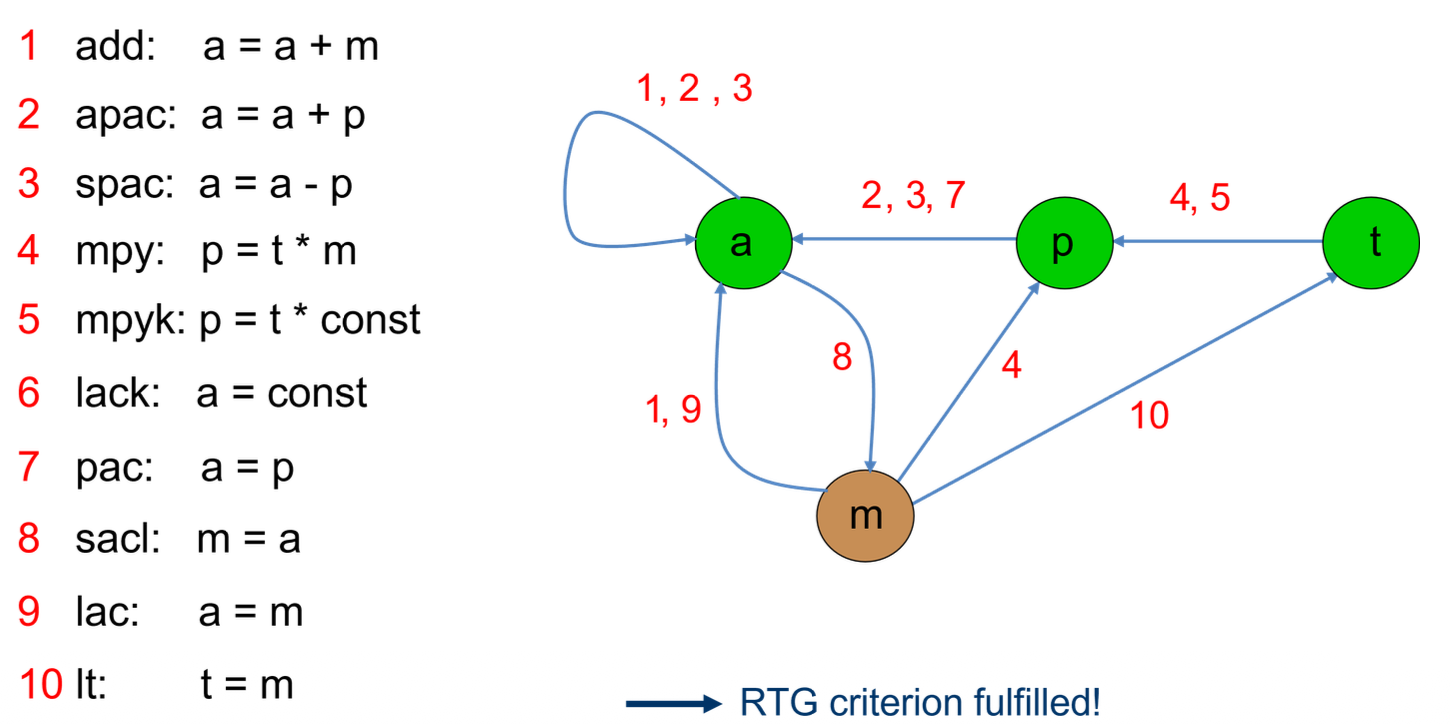
\includegraphics[width=0.5\textwidth]{images/RTG_criterrion.png}
		\caption{RTG for TMS320C25}
		\label{fig:RTG}
	\end{center}
\end{figure}

\subsection{Retargetable compiler}
\begin{itemize}
	\item Machine-independent compiler (automatically retargetable)
\begin{itemize}
	\item Compiler has built-in code generators for multiple targets
	\item Often used in parametric architecture 
\end{itemize}
	\item Compiler-Compiler (user retargetable)
\begin{itemize}
	\item Compiler is generated from a description of target architecture
\end{itemize}
	\item portable Compiler (developer retargetable)
\end{itemize}

\subsubsection{Processor Models}
\begin{itemize}
	\item Behavioral 
\begin{itemize}
	\item Describes the instruction set
	\item Relatively fast simulation possible
	\item Inaccuracy
\end{itemize}
	\item Structural
\begin{itemize}
	\item Describes the processor at RTL
	\item Accurate
	\item Simulation much slower
	\item Not always available
\end{itemize}
	\item Mixed models
\end{itemize}

\subsubsection{Tree-translation schemes}
\begin{itemize}
	\item Rules for transforming a syntax tree (resp. DAG)
\end{itemize}



 









